\documentclass[11pt]{article}
\usepackage[margin=1in]{geometry}
\usepackage[T1]{fontenc}
\usepackage{lmodern}
\usepackage{microtype}
\usepackage{amsmath}
\usepackage{booktabs}
\usepackage{tabularx}
\usepackage{enumitem}
\usepackage{xcolor}
\usepackage{tikz}
\usepackage{pgfplots}
\usepackage[colorlinks=true,linkcolor=accent,urlcolor=accent]{hyperref}
\pgfplotsset{compat=1.18}
\usetikzlibrary{arrows.meta,positioning}

\definecolor{accent}{HTML}{1F5FA8}
\definecolor{soft}{HTML}{EAF1FA}
\definecolor{warm}{HTML}{FFF4E0}
\setlength{\parindent}{0pt}
\setlength{\parskip}{0.6em}
\setlist{itemsep=0.2em,topsep=0.3em}
\newcommand{\cent}{\textcent}
\newcommand{\code}[1]{\texttt{#1}}
\tikzset{
  box/.style={draw=accent, fill=soft, rounded corners=2pt, minimum height=8mm,
              inner xsep=6pt, font=\small, align=center},
  arr/.style={-{Stealth[length=2.2mm]}, thick, accent}
}

\title{\textbf{A Market Maker on a Chip}\\[0.3em]
\large An LMSR prediction-market market maker built on an FPGA, in C++ and in Python}
\author{Dhanush Ekollu \quad MHacks}
\date{}

\begin{document}
\maketitle

\section*{The project in one paragraph}

We built a \emph{market maker}: a program that always stands ready to buy or
sell in a market, and keeps adjusting its prices as people trade with it. We
built the same market maker three times: as a digital circuit on an FPGA
board, as a C++ program, and as a Python program. All three give exactly the
same prices, down to the last bit, for the same sequence of trades. That lets
us compare them fairly on one question: how long does each take to produce a
new price, and how \emph{consistent} is that time?

This document explains the idea from scratch. No background in trading or
hardware is assumed.

\setcounter{tocdepth}{1}
\tableofcontents
\newpage

% ---------------------------------------------------------------------------
\section{Background: prediction markets and market makers}

\subsection{A prediction market}

A prediction market lets people trade on whether something will happen: ``Will
it rain in Ann Arbor on Friday?'' The thing being traded is a \textbf{YES
share}. A YES share pays \$1 if the event happens and nothing if it does not.

If a YES share is trading at 70\cent, the market is saying the event is about
70\% likely. Someone who thinks the real chance is 90\% would happily buy at
70\cent; someone who thinks it is 50\% would happily sell. The price moves
until buyers and sellers balance, so the price is a running estimate of the
probability.

\subsection{Why a market needs a market maker}

A market only works if there is someone to trade with. If you want to buy a
YES share and nobody happens to be selling at that moment, nothing happens.

A \textbf{market maker} solves this by always being available. At every moment
it posts two prices:

\begin{itemize}
  \item the \textbf{bid}: the price it will \emph{pay} to buy a YES share from you;
  \item the \textbf{ask}: the price it will \emph{charge} to sell a YES share to you.
\end{itemize}

The ask is always a little higher than the bid. The gap is called the
\textbf{spread}. If the market maker buys at 49\cent{} and sells at 51\cent{},
it earns 2\cent{} for providing the service of always being there.

\subsection{The market maker's problem}

Suppose many people buy YES from the market maker and few sell. It has now
sold a lot of YES shares. If the event happens, it owes \$1 on every one of
them. This pile-up is called \textbf{inventory}, and it is the market maker's
main risk.

A sensible market maker reacts by \emph{raising its prices} as it sells more.
Higher prices discourage further buying and encourage people to sell back,
which brings it back toward balance. Higher prices also reflect what the
buying is telling it: if everyone wants YES, YES is probably more likely than
the old price said.

So a market maker needs a rule that turns ``how much have I sold?'' into
``what should my bid and ask be now?'' Every time a trade happens it applies
the rule again and posts new prices. Doing this quickly matters: while its
prices are out of date, anyone who has noticed can trade against the stale
price.

% ---------------------------------------------------------------------------
\section{The pricing rule: LMSR}

We use a well-known rule called \textbf{LMSR} (logarithmic market scoring
rule), designed by the economist Robin Hanson for prediction markets. Its
appeal is that the market maker's whole memory is \emph{one number}.

\subsection{One number of state}

Let $d$ be the net number of YES shares the market maker has sold (sales minus
buy-backs). The fair price of a YES share is

\[
  p \;=\; \frac{1}{1 + e^{-d/b}} .
\]

This S-shaped curve is shown in Figure~\ref{fig:curve}. When $d = 0$ the price
is 50\cent. As the market maker sells more YES ($d$ grows) the price climbs
toward \$1, and as it buys YES back ($d$ falls) the price drops toward 0.

\begin{figure}[h]
\centering
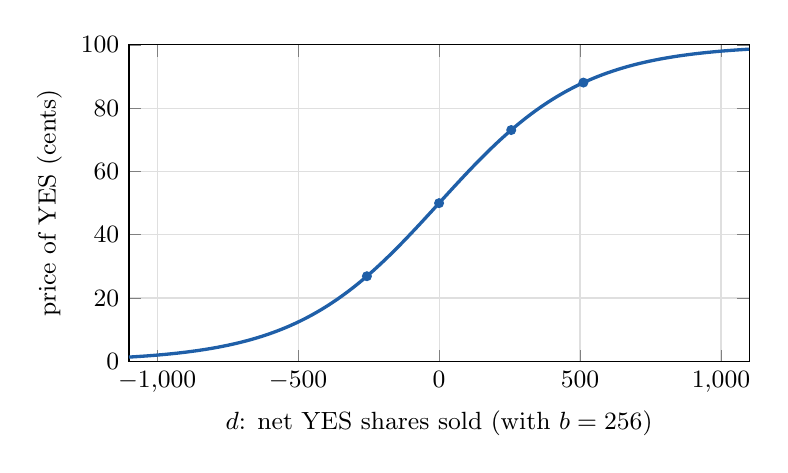
\begin{tikzpicture}
\begin{axis}[
  width=0.78\textwidth, height=5.6cm,
  xlabel={$d$: net YES shares sold (with $b = 256$)},
  ylabel={price of YES (cents)},
  xmin=-1100, xmax=1100, ymin=0, ymax=100,
  grid=major, grid style={gray!25},
  tick label style={font=\small}, label style={font=\small},
]
\addplot[accent, very thick, domain=-1100:1100, samples=120] {100/(1+exp(-x/256))};
\addplot[only marks, mark=*, mark size=1.6pt, accent] coordinates {(0,50) (256,73.1) (512,88.1) (-256,26.9)};
\end{axis}
\end{tikzpicture}
\caption{The LMSR price curve. Every 256 shares sold (one ``$b$'') moves the
price a fixed step along this curve: 50\cent{} $\to$ 73\cent{} $\to$ 88\cent.}
\label{fig:curve}
\end{figure}

\subsection{The liquidity setting $b$}

The number $b$ controls how quickly the price reacts. With a small $b$, a few
trades move the price a lot. With a large $b$, it takes many trades. It also
sets the most the market maker can ever lose, which is $b \ln 2$ dollars no
matter how anyone trades. For $b = 256$ that is about \$177. This cap is the
second big appeal of LMSR: the risk is known in advance.

\subsection{From the curve to a bid and an ask}

The market maker quotes for a fixed number of shares at a time, the
\textbf{quote size} $s$ (8 shares by default). LMSR defines a cost function
\[
  C(d) \;=\; b \,\ln\!\bigl(1 + e^{d/b}\bigr),
\]
and the price of a trade is the change in $C$. So:

\begin{align*}
  \text{ask} &= \frac{C(d+s) - C(d)}{s} && \text{(average price to sell $s$ more shares)}\\[0.3em]
  \text{bid} &= \frac{C(d) - C(d-s)}{s} && \text{(average price to buy $s$ shares back)}
\end{align*}

The ask comes out slightly above the fair price and the bid slightly below, so
a spread appears naturally. We then round the ask \emph{up} and the bid
\emph{down} to whole cents, so rounding never costs the market maker money.
Table~\ref{tab:quotes} shows what our market maker actually quotes.

\begin{table}[h]
\centering
\begin{tabular}{rccc}
\toprule
YES shares sold ($d$) & fair price & bid & ask \\
\midrule
$-256$ & 26.9\cent & 26\cent & 28\cent \\
$0$    & 50.0\cent & 49\cent & 51\cent \\
$128$  & 62.2\cent & 61\cent & 63\cent \\
$256$  & 73.1\cent & 72\cent & 74\cent \\
$512$  & 88.1\cent & 87\cent & 89\cent \\
$1024$ & 98.2\cent & 98\cent & 99\cent \\
\bottomrule
\end{tabular}
\caption{Quotes produced by our market maker ($b = 256$, quote size 8).}
\label{tab:quotes}
\end{table}

\subsection{The whole algorithm}

\begin{enumerate}
  \item Post a bid and an ask computed from $d$.
  \item A trader buys $q$ shares at the ask: set $d \leftarrow d + q$.\\
        A trader sells $q$ shares at the bid: set $d \leftarrow d - q$.
  \item Recompute the bid and ask from the new $d$ and post them. Repeat.
\end{enumerate}

Step 3 is the part we time. We call it \textbf{tick-to-quote}: the time from
learning about a trade to having the new prices ready.

% ---------------------------------------------------------------------------
\section{What we are comparing, and why}

\subsection{Why put this on an FPGA?}

An FPGA is a chip whose internal wiring can be reconfigured. Instead of
running a program one instruction at a time, you describe a circuit, and the
chip \emph{becomes} that circuit. Trading firms use FPGAs for two reasons:

\begin{itemize}
  \item \textbf{No operating system in the way.} A circuit reacts to its
        input directly. A program must wait for the operating system to hand
        it the data.
  \item \textbf{Perfectly repeatable timing.} A circuit takes the same number
        of clock ticks every time. A program's timing varies: another program
        interrupts it, or the data it needs is not in the processor's fast
        memory. This variation is called \textbf{jitter}.
\end{itemize}

\subsection{An honest expectation}

We are not claiming the FPGA is faster at the arithmetic. Our pricing step is
tiny, and a laptop processor runs billions of operations per second, while our
hobby-grade FPGA board runs at 12 million clock ticks per second. On the
\emph{typical} request we expect the C++ program to win.

The FPGA's advantage is consistency. In trading, the slow cases matter most:
the one request in a thousand that takes far longer than usual is exactly when
a market maker's prices are out of date. A design whose worst case equals its
typical case has no such moments. That is the result this project is built to
show.

\subsection{Keeping the comparison fair}

\begin{itemize}
  \item \textbf{Identical answers.} All three versions follow one written
        specification and must agree bit for bit, so none can be faster by
        doing less work.
  \item \textbf{Identical input.} One fixed file of trades is replayed into
        all three.
  \item \textbf{Compute time only.} Each version measures itself from ``the
        whole request has arrived'' to ``the new prices are ready'', and
        reports that number inside its reply. The time spent moving bytes
        between the laptop and the market maker is left out for all three.
\end{itemize}

% ---------------------------------------------------------------------------
\section{Making the math fit in hardware}

The formulas above use logarithms, exponentials, multiplication and division.
Our FPGA has none of these built in, not even a multiplier. Each design
decision below removes one obstacle.

\begin{table}[h]
\centering
\renewcommand{\arraystretch}{1.25}
\begin{tabularx}{\textwidth}{>{\raggedright\arraybackslash}p{0.27\textwidth}X}
\toprule
\textbf{Decision} & \textbf{Why} \\
\midrule
Whole numbers only, no decimals &
Decimal (floating-point) arithmetic can round differently in different
languages. Whole numbers behave identically everywhere, so the three versions
can match exactly. Prices carry 16 extra binary digits of precision
internally. \\
A lookup table for the hard function &
$\ln(1+e^{x})$ is too expensive to compute in a small circuit. It equals a
straight line plus a small bump that fades to zero, so we store only the bump:
2{,}048 precomputed values. Looking up a value replaces computing it. \\
Powers of two for $b$ and $s$ &
$b$ is 64, 128 or 256, and $s$ is a power of two no larger than $b$.
Multiplying or dividing by a power of two is just shifting digits, which costs
almost nothing in hardware. It also lets one table serve every setting. \\
Round in the market maker's favour &
Ask rounds up, bid rounds down, to whole cents. Before rounding, the
whole-number price is within 0.004\cent{} of the exact formula. \\
Stop quoting instead of forcing a price &
If the ask would exceed 99\cent{} (or the bid fall below 1\cent), that side of
the quote is withdrawn. Forcing the price back into range would mean trading
at a price worse than the rule allows. \\
\bottomrule
\end{tabularx}
\end{table}

With these choices, one new quote costs three table lookups, two subtractions,
and some shifting and rounding. Nothing else.

% ---------------------------------------------------------------------------
\section{The system}

\begin{figure}[h]
\centering
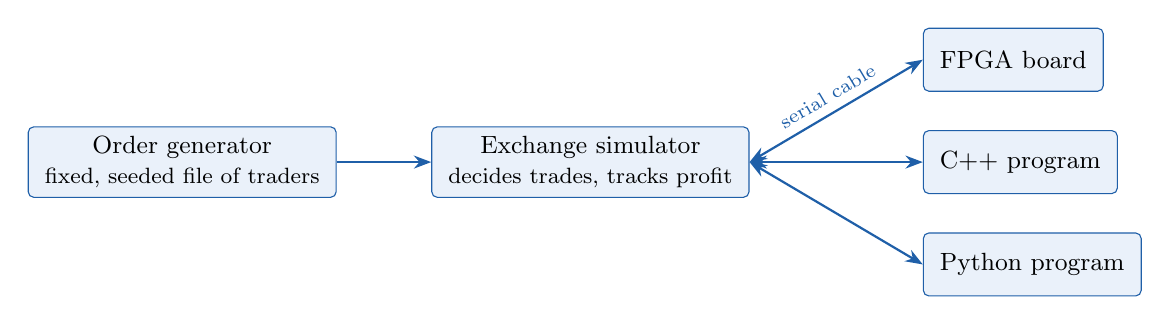
\begin{tikzpicture}[node distance=7mm and 12mm]
  \node[box] (gen) {Order generator\\\footnotesize fixed, seeded file of traders};
  \node[box, right=of gen] (ex) {Exchange simulator\\\footnotesize decides trades, tracks profit};
  \node[box, right=22mm of ex, yshift=13mm] (fpga) {FPGA board};
  \node[box, right=22mm of ex] (cpp) {C++ program};
  \node[box, right=22mm of ex, yshift=-13mm] (py) {Python program};
  \draw[arr] (gen) -- (ex);
  \draw[arr, {Stealth[length=2.2mm]}-{Stealth[length=2.2mm]}] (ex.east) -- node[above, sloped, font=\scriptsize]{serial cable} (fpga.west);
  \draw[arr, {Stealth[length=2.2mm]}-{Stealth[length=2.2mm]}] (ex.east) -- (cpp.west);
  \draw[arr, {Stealth[length=2.2mm]}-{Stealth[length=2.2mm]}] (ex.east) -- (py.west);
\end{tikzpicture}
\caption{The same trades are replayed into each of the three market makers.}
\end{figure}

\subsection{Simulated traders}

The order generator writes a file of trader arrivals from a random seed, so
the same seed always gives the same file. There is a hidden ``true''
probability that the market maker cannot see. Two kinds of trader arrive:

\begin{itemize}
  \item \textbf{Noise traders} buy or sell at whatever the current price is.
        They are the market maker's source of income, because they pay the
        spread.
  \item \textbf{Informed traders} know the true probability. They buy only
        when the ask is below it and sell only when the bid is above it. They
        cost the market maker money, but they are also what pulls its price
        toward the truth.
\end{itemize}

The true probability can jump partway through (``news''), and we watch the
market maker's price follow it.

\subsection{The exchange simulator}

The exchange reads the file one trader at a time, looks at the market maker's
current bid and ask, decides whether that trader trades, tells the market
maker, and reads back the new prices. It keeps the books: the market maker's
inventory, its cash, and its profit or loss.

\subsection{The messages}

The exchange and a market maker talk in short fixed-size messages. A request
is 5 bytes (for example ``a trader bought 8 shares''). A reply is 13 bytes:
the new bid and ask, the inventory, a running count of trades, and how long
the computation took. Each message ends with a checksum so a corrupted one is
detected and ignored.

% ---------------------------------------------------------------------------
\section{The FPGA design}

The board is a ``HailBoard'' with a Lattice iCE40 HX4K FPGA: a small,
inexpensive chip with no multipliers and about 16 kilobytes of on-chip memory.
It talks to the laptop over a serial link at 115{,}200 bits per second. The
design is written in Verilog, a language for describing circuits.

\subsection{The pipeline}

The circuit is a chain of small modules. Bytes arrive from the laptop, become
a request, get priced, and leave as a reply.

\begin{figure}[h]
\centering
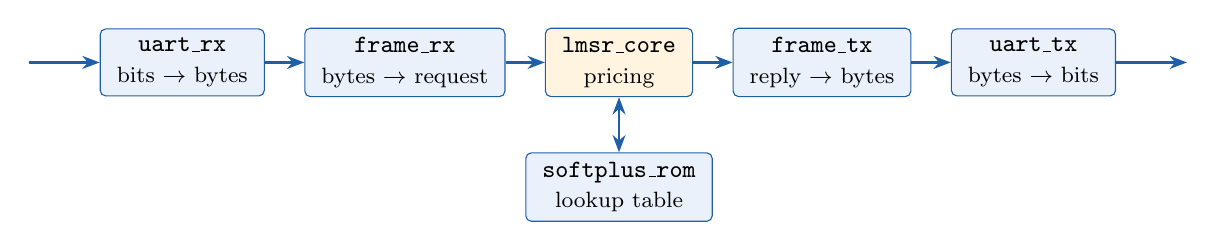
\begin{tikzpicture}[node distance=5mm]
  \node[box] (rx)  {\code{uart\_rx}\\\footnotesize bits $\to$ bytes};
  \node[box, right=of rx]  (frx) {\code{frame\_rx}\\\footnotesize bytes $\to$ request};
  \node[box, right=of frx, fill=warm] (core) {\code{lmsr\_core}\\\footnotesize pricing};
  \node[box, right=of core] (ftx) {\code{frame\_tx}\\\footnotesize reply $\to$ bytes};
  \node[box, right=of ftx] (tx) {\code{uart\_tx}\\\footnotesize bytes $\to$ bits};
  \node[box, below=7mm of core] (rom) {\code{softplus\_rom}\\\footnotesize lookup table};
  \draw[arr] (rx) -- (frx); \draw[arr] (frx) -- (core);
  \draw[arr] (core) -- (ftx); \draw[arr] (ftx) -- (tx);
  \draw[arr, {Stealth[length=2.2mm]}-{Stealth[length=2.2mm]}] (core) -- (rom);
  \draw[arr] ([xshift=-9mm]rx.west) -- (rx.west);
  \draw[arr] (tx.east) -- ([xshift=9mm]tx.east);
\end{tikzpicture}
\caption{The modules of the FPGA market maker.}
\end{figure}

\begin{table}[h]
\centering
\renewcommand{\arraystretch}{1.2}
\begin{tabularx}{\textwidth}{>{\raggedright\arraybackslash}p{0.2\textwidth}X}
\toprule
\textbf{Module} & \textbf{What it does} \\
\midrule
\code{uart\_rx} & Reads the serial wire and assembles bits into bytes. It
finds the start of each byte and then samples the middle of every bit, where
the signal is most stable. \\
\code{frame\_rx} & Collects 5 bytes into a request and checks the checksum. If
a message stalls halfway, it gives up after 10 milliseconds so one lost byte
cannot jam the link. \\
\code{softplus\_rom} & The lookup table, held in the chip's block memory. \\
\code{lmsr\_core} & The market maker itself: it holds $d$, the settings and the
current prices, and computes new prices after each request. \\
\code{frame\_tx} & Packs the reply into 13 bytes and hands them out one at a time. \\
\code{uart\_tx} & Sends each byte down the serial wire, bit by bit. \\
\code{top} & Connects everything, reads the buttons, drives the displays, and
counts how many clock ticks each request takes. \\
\bottomrule
\end{tabularx}
\end{table}

\subsection{Inside the pricing core: seven clock ticks}

A digital circuit advances in steps driven by a clock; ours ticks 12 million
times a second. The pricing core handles every request in exactly seven ticks:

\begin{enumerate}
  \item Apply the request: update $d$ for a trade, or change a setting.
  \item Ask the table for the value at $d - s$.
  \item Ask for the value at $d$. The first answer arrives and is saved.
  \item Ask for the value at $d + s$. The second answer arrives.
  \item The third answer arrives.
  \item Subtract: the upper difference gives the ask, the lower gives the bid.
  \item Shift, round to cents, add any extra spread, and decide whether each
        side should be withdrawn.
\end{enumerate}

The three lookups happen on separate ticks because the chip's memory answers
one question per tick. Splitting the work into small steps also keeps each
step short enough to finish comfortably within one tick.

One more tick is spent checking the incoming message, giving \textbf{8 ticks
in total, or 667 nanoseconds}, for every request without exception. There is
no branch in the circuit that could make one request take longer than another.

\subsection{Board controls}

The eight-digit display shows the bid, the ask, and the number of trades so
far. Four push buttons control a live demonstration:

\begin{center}
\begin{tabular}{ll}
\toprule
Button & Action \\
\midrule
KEY0 & Restart the market maker and replay the trades from the beginning \\
KEY1 & Kill switch: withdraw all prices immediately (press again to resume quoting) \\
KEY3 & Pause the stream of trades at the current one \\
KEY2 & Resume the stream \\
\bottomrule
\end{tabular}
\end{center}

A \textbf{kill switch} is a standard safety feature of real trading systems:
one control that stops all quoting at once if something looks wrong, without
erasing the current position. The trades themselves are stored on the laptop,
so the restart, pause and resume buttons work by sending a short message to
the laptop program that feeds the board.

% ---------------------------------------------------------------------------
\section{Results so far}

Everything in this section has been measured. Nothing is estimated.

\begin{itemize}
  \item \textbf{Accuracy.} Across all 60{,}392 combinations of settings and
        inventory, the whole-number price differs from the exact formula by
        at most 0.0038\cent{} before rounding to cents.
  \item \textbf{Identical behaviour.} A set of 6{,}971 test requests, chosen
        to exercise every rule (price limits, bad sizes, the kill switch,
        every setting), produces identical replies from the FPGA board, the
        C++ program and the Python program.
  \item \textbf{Identical trading runs.} Four full simulated markets, between
        1{,}290 and 3{,}297 trades each, produce byte-for-byte identical
        streams of prices from all three.
  \item \textbf{FPGA timing.} On the real board, every one of those replies
        reported a compute time of exactly 8 clock ticks (667 ns).
  \item \textbf{Size.} The design uses 1{,}546 of the chip's 7{,}680 logic
        cells and 12 of its 32 memory blocks. The tools estimate it could run
        at about 49 million ticks per second, four times the speed it needs.
\end{itemize}

The FPGA design was first checked in simulation, where a test program plays
the role of the laptop and compares every reply against the Python reference,
and only then loaded onto the board and checked again.

\subsection*{What comes next}

\begin{itemize}
  \item \textbf{The latency benchmark.} Run all three at the same pace, record
        the full distribution of compute times (typical, 99th percentile,
        99.9th percentile, worst), and repeat with the laptop under heavy
        load. This produces the jitter comparison that is the point of the
        project.
  \item \textbf{Demonstration polish.} Decimal prices on the display, switches
        to change settings, and a dashboard plotting the market maker's price
        against the hidden true probability, together with its inventory and
        profit.
\end{itemize}

\end{document}
